\chapter{Related Work}

The importance of video service in the cloud is considerable due to lot amount of video information transferred over networks. Recently, video cloud has become a hot research topic. The compressed video sensing (CVS) and sparse representation is an alternative that is gaining strength thanks to the results of compressive sensing (CS) in fields as image/video reconstruction, image/video super-resolution and image/video compression. For video coding with sparse representation, Shen \emph{et al}. in \cite{motion_cs} propose to perform the motion estimation based in sparse representation. A region $C$ denotes the current block to  be predicted and a region $S$ denotes the neighbour blocks of $C$.  search a good approximation for know pixels in a $S$ region and its sparse representation coefficient is calculated and then keep the same procedure to estimate the unknown pixel value in $C$ region. In this proposal two dictionary are used, $D_S$ for pixel of region $S$ and $D_C$ for pixel of region $C$. Sparse representation is calculated with OMP algorithm and energy of residual on the current block is used as the stopping criteria. In \cite{odl_me}, Sun \emph{et al}. propose a framework for inter-frame video coding using sparse representation with online dictionary learning. The dictionary is training with textured patches of each frame in the video in order to obtain sparse representation for the following frames. Furthermore, the sparse coefficients are quantized and encoded using Huffman entropy encode. A module is added in the encoder for construct the sparse representation and another is added the decoder for reconstruct the image. The framework was compared with H.264 video encoder and  K-SVD dictionary, showing better rate distortion performance but increasing the bit rate the performance gradually decrease. \\

For the other hand, Xiong \emph{et al}. in \cite{sparse_st, 6189245} use sparse representation for up-sampling video frame in low resolution. Key frames are selected as high resolution and the non-key frame are down-sampled in low resolution. High resolution version are recovered  using the learning-based super-resolution reconstruction and all frames of the video are encoded and decoded using H.264 encoder. For reconstruction a set of 2-D sub-dictionary pairs (High Resolution and Low resolution) and a 3-D dictionary pair (High Resolution and Low resolution) are created. First dictionary is trained with primitive frame patches and the second dictionary is trained with interpolated patches combined with the most matched patches in the neighbour training frame using K-SVD algorithm. This proposal shows improvements in coding efficiency in low bit-rate regions compared to H.264 encoder. The figure \ref{fig:spatio-temporal} show the learning framework of sparse spatio-temporal representation for video coding. \\

\begin{figure}[!h]
\centering
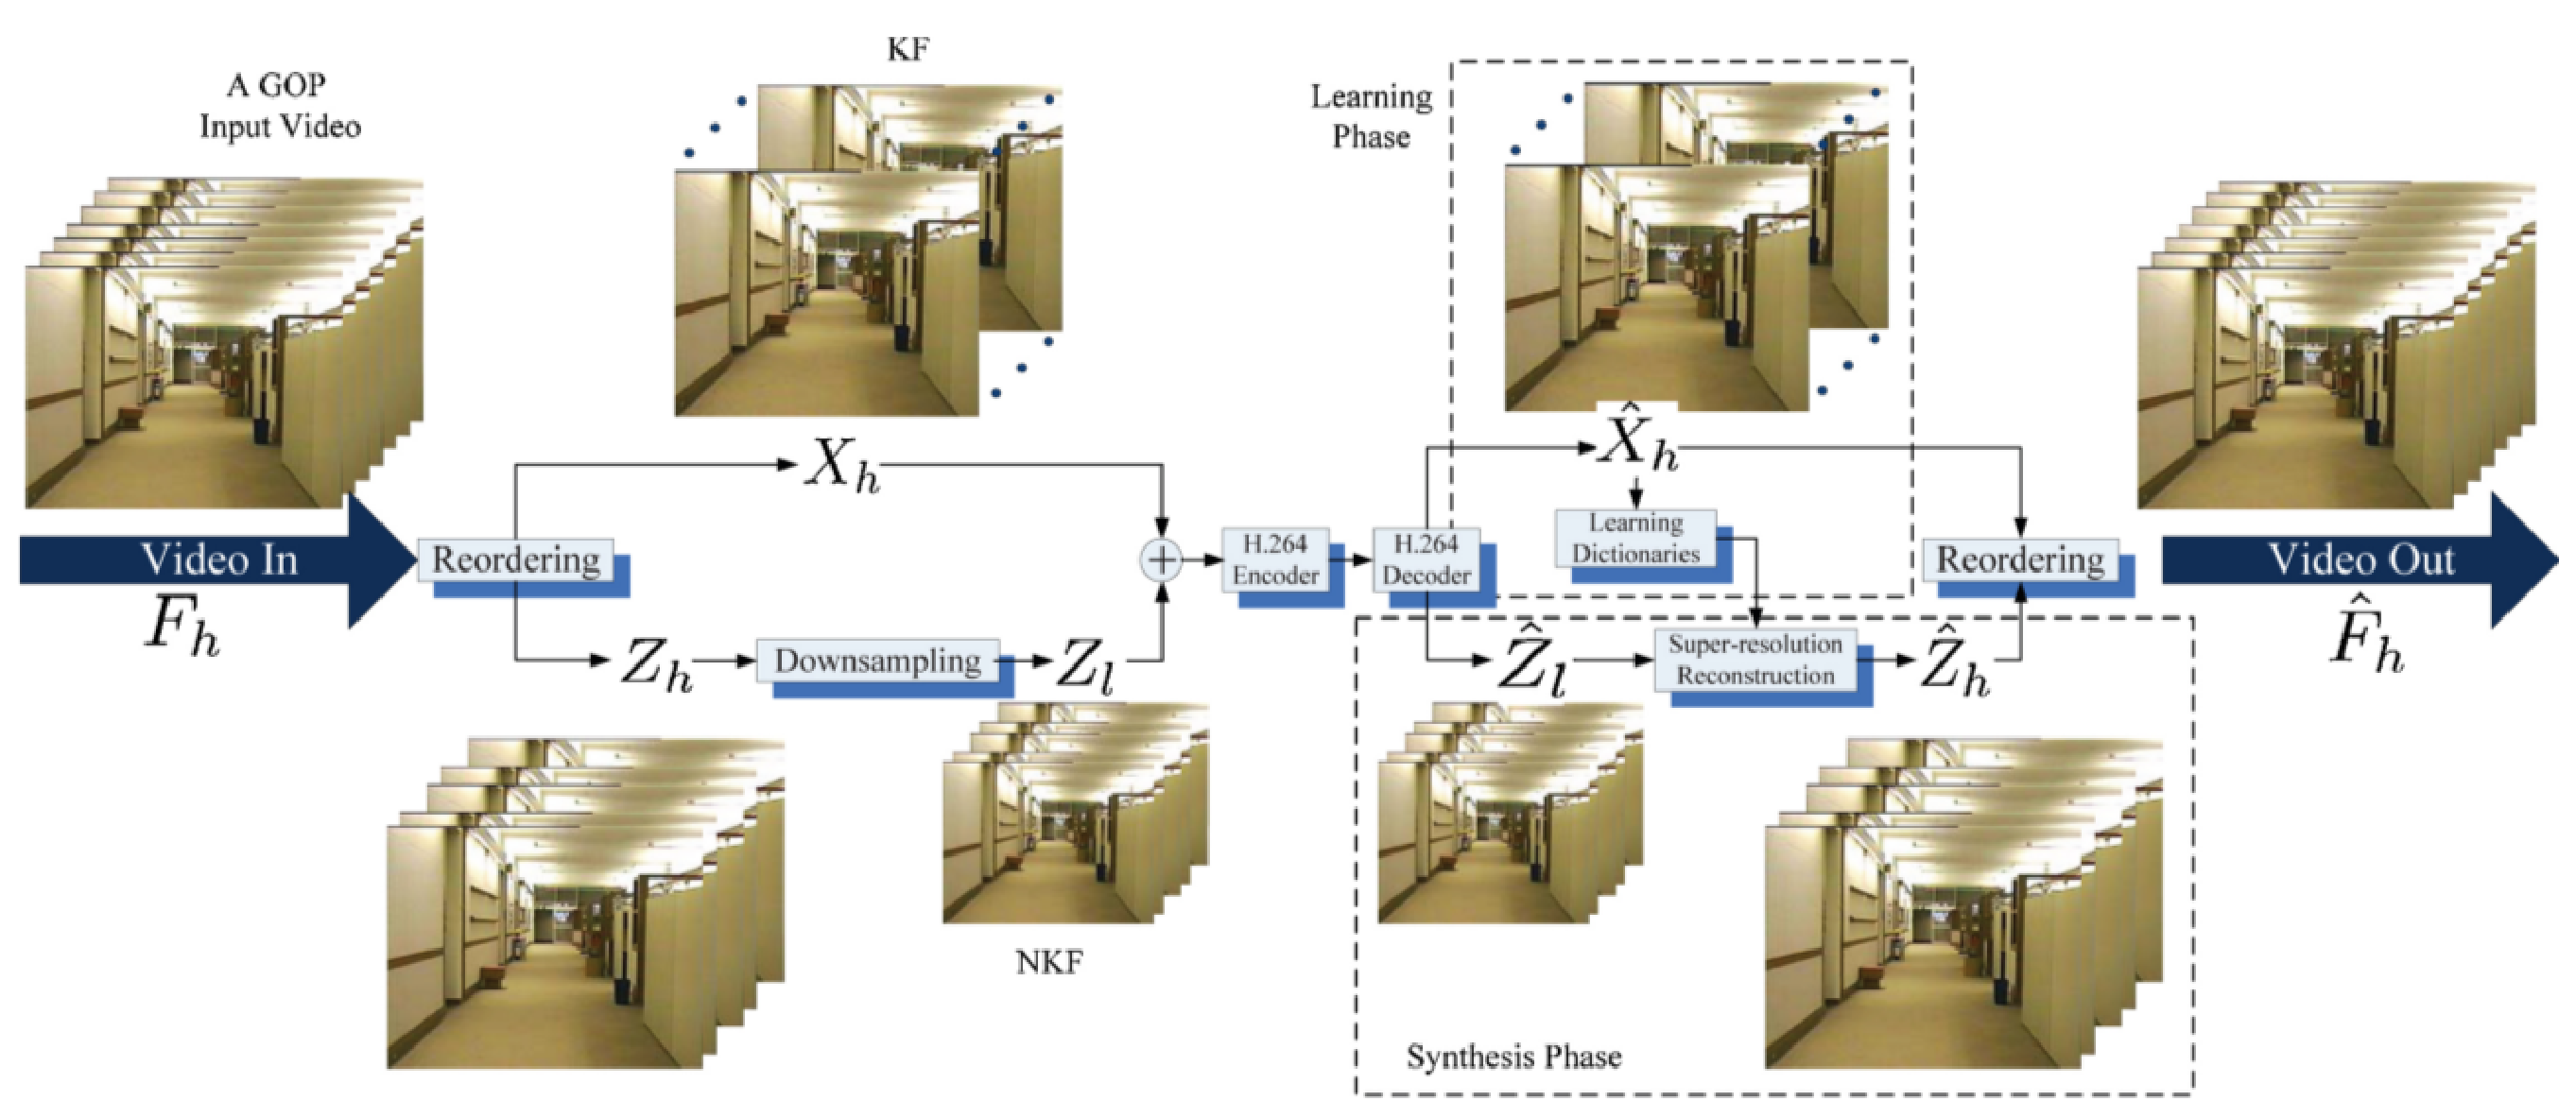
\includegraphics[width=\textwidth]{images/spatio-temporal.eps}
\caption[Learning framework of sparse spatio-temporal representation for video coding]{Learning framework of sparse spatio-temporal representation for video coding \cite{sparse_st}}
\label{fig:spatio-temporal}
\end{figure} 

In the field of compressed video sensing, Azghan \emph{et al}. present in \cite{7076640} a compressive sampling and  multihypothesis reconstruction strategy for video sequences. The video frames are grouped as reference and non-reference. Reference frame is divided into non-overlapping blocks and it are vectorized row-wise, compressively sensed and sent to the  decoder. For each block of the non-reference frames, the corresponding dictionary  is  constructed  by  stacking  (column-wise)  a number  of  vectorized  blocks  of  the  reference frame that are lying inside the search window. At the decoder side, the current block is recovered,  knowing that the current block is sparse in the discrete cosine  transform (DCT) domain using multihypothesis technique (motion estimation task is performed by the decoder instead of encoder). The proposed approach is compared with Multihypotheis Elastinec algorithm \cite{Chen:2015}, obtained  a increasing in PSNR of 1.19 dB on average. In \cite{6984694}  Guo \emph{et al}. propose a new motion estimation method in measurement domain for CVS. This proposal is based on the correlation relationship to  
estimate the measurements of a block in a random unknown position in a frame, taking advantage of measurements of the adjacent non-overlapping blocks. The current block is formulated as a linear combination  of the four non-overlapping blocks using sparse representation. \\
 
In some articles combine the distributed video coding (DVC) with compressing sensing, in a proposal called Distributed Compressed Video Coding (DVCS). DVC avoids the computationally intensive temporal prediction  loop at the encoder, by shifting the exploitation of the temporal redundancy to the decoder \cite{5202822} . For DVCS,  Baig \emph{et al}.propose in \cite{6266276} a codec entirely based on CS. Video frames are divided into key frames and non-key frames and are converted to a column vector for calculate the CS measurements. The calculated measurements are quantized using Gaussian quantization. In the decoder side, each key frame is reconstructed with sparse representation. A dictionary is constructed with CS measurements of key frames available at the decoder for reconstructing the non-key frame based on the correlation between its CS measurements and the dictionary. In \cite{6245804} Yu \emph{et al}. propose a multiple description distributed compressed video sensing. In the multiple description, the video sequence is split into two subsequences (two   descriptions) and compressed with almost the same quality  but  transmitted  over  two  different channels, when all descriptions are received, the central decoder will work to provide  the  best  quality  reconstruction  of  the  video  sequence. At the encoder, the original video sequence is split into key-frame followed by some CS frames and all are compressed by CS method generating two descriptions. The strong  correlation among frames allows that measurement rate of CS-frames can be lower than that of key-frames. Additionally the complexity is reduce using block-level CS. At the decoder, key-frames are recovered by simply applying the block-level CS reconstruction, while for the CS-frames, the CS process is improved by a motion estimation. If all descriptions are received, the decoder central can structure CS frames by searching temporal neighbouring blocks from previously recovered adjacent key-frames using more sparse domains for reconstruction taking advantage of the temporal correlation that exists in the video signal. \\

In the case of cloud-based proposal using CS, Wang \emph{et al}. in \cite{6694139} propose a cloud-based compressive sensing video communication system. The system proposed mainly includes video senders, cloud platform and receivers. The encoder receives the raw samples and generates compressed video frames with CS using block Hadamard of 32 $times$ 32 for construct the dictionary. Video sequence are divided in $I$ frame which are directly compressed and $P$ frame which are encoded by utilizing the temporal redundancy between  adjacent frames. $I$ frame are taken as image reference frame, while $P$ frames are constructed by taking CS scheme of algebraic difference with its closest $I$ frame represented by a vector. For combating the data loss in wireless networks, a CS erasure code (CSEC) adaptive based on bit error rate is proposed. Adaptive error detecting schemes are used in different channel conditions, and  CSEC is combined to compensate for the quality degradation resulted from channel error. The CS-reconstructed video is transcoded to H.264-encoded video streams in the cloud platform and finally transmitted to the receiver. \\

\begin{figure}[!h]
\centering
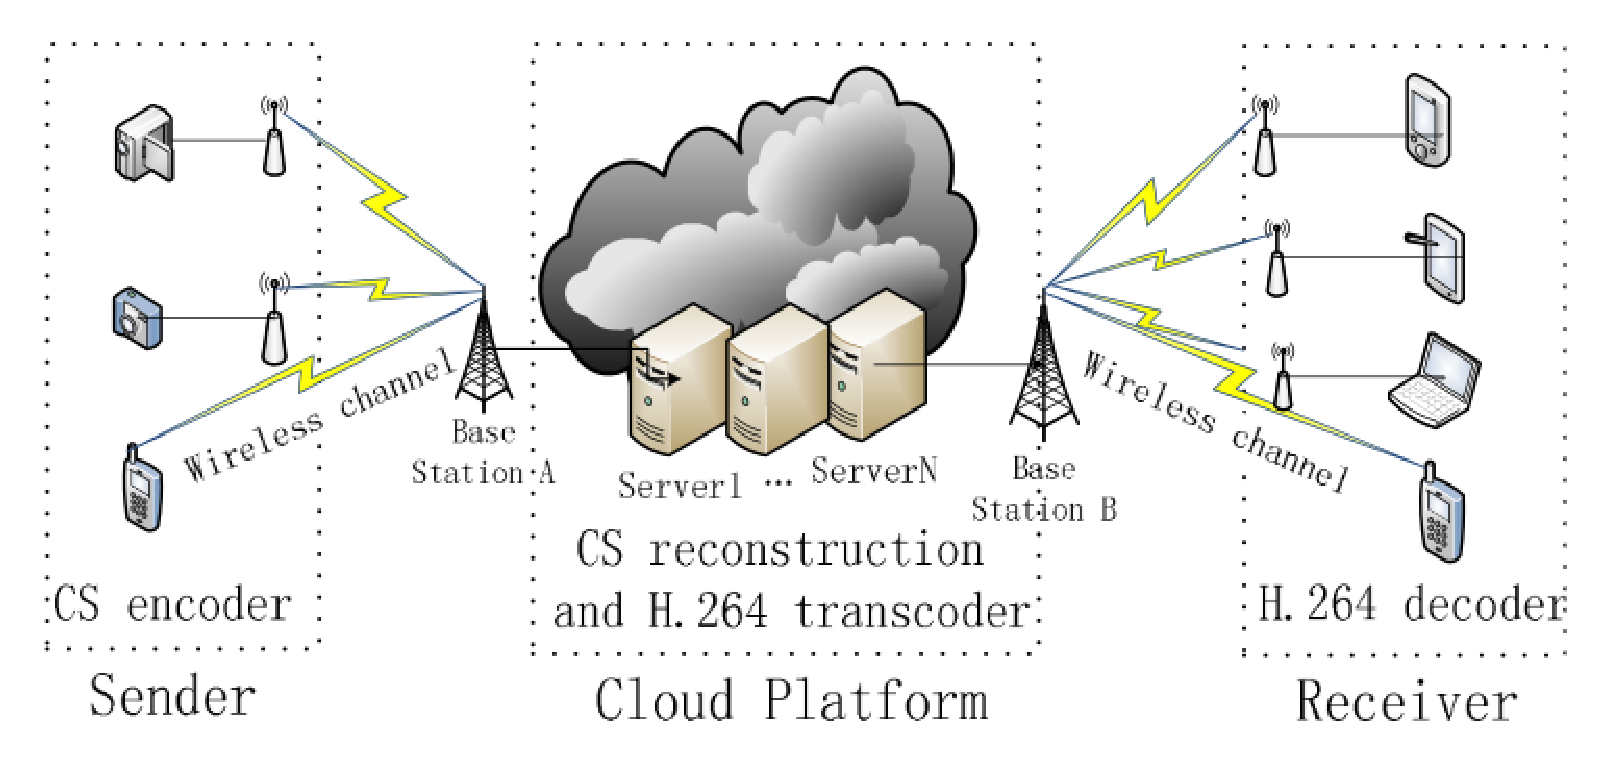
\includegraphics[width=0.6\textwidth]{images/cloud-based.eps}
\caption[Cloud-based compressive sensing video transmission system]{Cloud-based compressive sensing video transmission system \cite{6694139}}
\label{fig:cloud-based}
\end{figure} 